Das Klimasystem ist ein komplexes und hoch-dimensionales System. Dieses durch ein Modell berechenbar zu machen ist dementsprechend schwierig und bedarf einiger Abstraktionen. Laut Definition \cite[vgl.][]{stachowiak} sollen Modelle nicht alle Attribute des abgebildeten Systems übernehmen sondern vielmehr eine Vereinfachung dessen sein mit einer kleinst-möglichen und aber notwendig großen Komplexität. Auf Klimamodelle bezogen, bedeutet dies, dass man nicht alle Faktoren in das Modell miteinbeziehen kann und daher manche durch Parameter und Annäherungen abgebildet werden müssen. Ein globales Klimamodell (\textbf{GCM}) liefert im generellen recht gute Aussagen über die Entwicklung des globalen Klimas, jedoch beruhen diese Ozean-Atmosphären gekoppelten Zirkulationsmodelle, auf einer Parametrisierung der Konvektion, da diese im relativ groben Raster eines GCM nicht simuliert werden kann. Dadurch können grobe Fehler entstehen. \cite[vgl.][Stevens \& Bony]{stevensbony}. Jedoch ist aufgrund der Rechenkosten und Rechenzeit eine solche Herangehensweise mit parametrisierter Konvektion im simulieren großflächiger (globaler) Klimamodelle  unumgänglich. Da in fast allen GCMs durch die Parametrisierung die dynamischen Prozesse der Atmosphäre wie z.B. der Polare Jet, die nordatlantischen Stürme oder auch die stationären planetaren Wellen durch stark vereinfachte empirische Modelle abgebildet werden, müssen viele BIAS-korrigiert werden. Dadurch sind diese GCMs eine starke Fehlerquelle der Regionalen Klimamodelle, da sie als Input für ebendiese genutzt werden. (vgl. \cite{woollings_2013})\\
Um akkurate Aussagen über die Klimaveränderung basierend auf GCMs zu tätigen muss das grobe globale Klimamodell auf ein feineres Raster gebracht werden. Da auf dieser fein skalierten Ebene die Ortographie (wie z.B die Alpen oder die Pyrenäen), die flache (shallow) Konvektion, die zu Tiefenkonvektion wird und die lokalen Kältepools große Auswirkungen auf die Wettererscheinungen haben müssen diese variablen entweder statistisch parametrisiert oder dynamisch berechnet werden. Diese Vereinfachungen sind wieder eine große Fehlerquelle für Vorhersagen (vgl. \cite{maraun_2010,casanueva_2013}). Zudem kommen noch etwaige Rückkopplungen des regionalen Klimas auf das Globale hinzu, was zu einer weiteren Fehlerquelle führen kann. Wie man in der Publikation von Teixera et al.\cite{teixeracardoso} und Chen et al.\cite{chenshuyi} lesen kann hat die flache Konvektion durch die starke Rückwirkungen auf die Tiefenkonvektion auch eine Auswirkung auf das globale Klima, wie es z.B. gut Anhand der Tropen  und der Madden-Julian Oszillation zu erkennen ist, wo aus flacher Konvektion Tiefenkonvektoin wird und daraus sich großflächige Wettererscheinungen bilden. Zudem sollte hier angeführt werden, dass auch die Auflösung von gegenwärtigen Klimamodelle nicht immer ausreichend ist: z.B. können Turbulenzen und andere atmosphärische Mikroprozesse nicht von der derzeitigen ''Standard-''Maschenweite der Simulationsgitter vollends erfasst und müssen, um grobe Fehler zu vermeiden, statistisch und dynamisch kombiniert \glqq downgescaled\grqq \ werden. \cite[vgl.][Maraun et al.]{marauntowards}\\
Aufgrund dieser Rückwirkung der regionalen Klimamodelle (\textbf{RCM})auf die GCM's stellt sich auch die Frage, ob denn gegenwärtige globale Klimamodelle bereit sind, sie als Datenquelle für RCM's zu verwenden.\\
Als letzte größte Fehlerquelle für Klimamodelle wird die interne Variabilität des Klimas angeführt \cite[vgl.][]{maraun_2013}. ''Jede extern (Mensch oder astronomische Erscheinungen) getriebene Klimareaktion wird von internen Klimafluktuationen überlagert. Die Amplitude dieser Fluktuationen hängt von der betrachteten Variable, der Region und der Saison ab. Im Kontrast zu den Modellfehlern, können dies nicht bis auf die Zeitskala ihrer Vorhersage reduziert werden. Deshalb könnte ein hypothetisch perfektes Klimamodell auch nicht mehrjährige Vorhersagen treffen, die nicht von zufälligen Fluktuationen dominiert sind. Dies betrifft besonders die regionalen Klimamodelle'' (frei übersetzt nach \cite{maraun_value}, Seite 3).\newline
\begin{figure}[h]
	\centering
	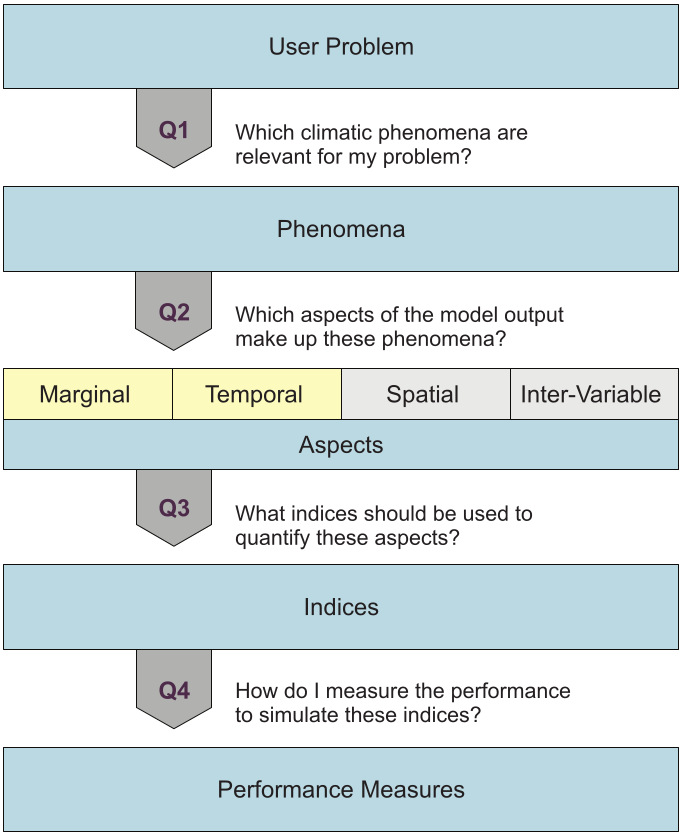
\includegraphics[width=0.5\textwidth]{VALUE.png}
	\caption{Baumstruktur, um eine geeignete Evaluationsmethode zu finden von Maraun et al. in VALUE \cite{maraun_value}}
	\label{fig:value}
\end{figure}

Um nun eine geeignete Evaluierungsmethode zu finden halte ich mich an die Grafik in Abb. \ref{fig:value}. Die Fragen werden nun hier strukturiert beantwortet:
\begin{itemize}
	\item Q1: Starkregenereignisse, und Übereinstimmung von Niederschlagsmuster im Allgemeinen
	\item Q2:
		\subitem{*} Marginal: Intensität
		\subitem{*} Temporal: Jahreszeit bzw. Dauer der Erscheinungen.
		\subitem{*} Spatial: Gewitterzellen sind auf kleinen Arealen zu finden (in den Alpen)
		\subitem{*} Inter-Variable: Temperatur als Begleiterscheinung bei Gewittern.
	\item Q3: Mittelwert der Niederschläge, 99. Quantile, Jahreszeiten, Temperatur-Niederschlagskorrelation, Übereinstimmung der Verteilungskurven und damit dem BIAS der Kurven, räumliche Übereinstimmung mit den Beobachtungsdaten.
	\item Q4: BIAS und relative Fehler (zu den Beobachtungsdaten)
\end{itemize}

Um nun die beiden Klimamodelle möglichst weitgehend miteinander zu vergleichen werde ich sie über den Mittelwert des Niederschlags, das 99. Quantil über alle zehn Jahre und das 99.Quantil in den vier Jahreszeiten mit den Beobachtungsdaten vergleichen. Welche Vor und Nachteile diese Methoden mit sich bringen habe ich im Kapitel \ref{chap:methods} angeführt.\\



